\section{Introduction}
\label{sec:intro}

% %Problem
% The current LLM benchmarks are broken due to the following problems
% 1) Most benchmarks use reused, unhidden test sets.
% 2) It is not easy to detect contamination or overfitting.
% 3) The growth speed of model capability exceeds the growth speed of benchmark building. The model capability is very general now.
% 4) There is a significant gap between benchmark and real-world performance
% 5) Benchmark scores are very sensitive to prompt formats.

% % Some reasons
% These problems are more severe for LLMs because
% 1) LLMs are extremely good at memorizing and capable of minor generalizations.
% 2) The training data of LLMs are not restricted. People crawl data from all possible sources and distill it from strong models. People compete on data instead of model architecture.

% % The current bad situation
% These issues lead to a very bad situation currently
% 1) Model developers and companies sell their models by showing high benchmark scores (e.g., MMLU).
% 2) Open-source model developers compete on the Huggingface OpenLLM leaderboard.
% 3) No one can trust benchmark scores anymore, which diminishes the value of benchmarks.

% % Our methods and results
% We show such vulnerability can be exploited intentionally, or it might occur unintentionally.
% Our models achieve XXX GSM-8K, XXX MMLU, and XXX HumanEval scores without being detected by major contamination detection algorithms.

% % Next
% We suggest that future LLM benchmarks should adopt a one-time exam approach.


% Currently, the LLM landscape is evolving rapidly. More and more people are getting involved in LLM model development, and many have made significant efforts toward LLM evaluation benchmarks. Some models have achieved very high scores on benchmarks, even surpassing OpenAI's GPT-4. However, in practical use, some models do not demonstrate capabilities corresponding to their benchmark performance. The reason for this discrepancy is that the current LLM benchmarks are, to some extent, failing.

%\ion{Say the contamination is a big problem. Then, there are two possible solutions (a) detect that a model is contaminated and the benchmark results cannot be trusted, or (b) we need one-time exams, i.e., new tests that were never published before so that the chance of the models contaminated with the test questions is very low. With (a) actually the problem is what do you do with the information that the model is contaminated? Of course, you won't trust the benchmark, but the model can still be very good for your task. People still won't ignore it. And the cost of remediation is huge, i.e., identifying and removing the contaminated data from the dataset and then retraining (which can be hugely expensive). Of course, with (b) it is very hard to come up with totally new exams, but this is the challenge we pose to the community. 
%Maybe one way to turn around the argument is to we use the contamination tests to make sure that the chance of the one-time exam being contaminated is low.
%Just to be very clear. A paper focusing on the contamination attacks and defenses is a good paper. I am not opposed at all writing this paper. But if we focus on the attacks, this is not the paper to argue that "benchmarks are broken and we need one-time tests". That is a different paper, and it is ok to write both.
%Also another thing to be clear about. In the "benchmarks are broken and we need one-time tests" paper, we do not need to come with the bullet-proof solution. We need only to be successful in arguing that the current benchmarks are broken, and then that one-time test is a possible solution (which should be easy). The final solution is a call for action to the community. 
%}

% \weilin{
% \begin{enumerate}
%     \item LLM’s capability is progressing more rapidly than ever. However, people still use static benchmarks to evaluate LLMs
%     \item There is strong evidence that many benchmarks may have been contaminated. (cite GPT-4, Llama, PaLM)
%     \item What's worse, most models are released without ANY contamination analysis. Without access to training data, it’s almost impossible to examine whether a model is contaminated. We have no clue whether we are really making progress. The culture is bad.
%     \item Even with data access, we still lack of effective tools to detect contamination
%     \item In this work, we show that a simple rephrase technique can contaminate the dataset without being detected by existing detection methods.
%     \item We propose a stronger contamination test and urge the community to adopt the tool before reporting any benchmark numbers.
%     \item To fundamentally resolve the issue, we call for the community to evaluate LLMs with one-time exams.
% \end{enumerate}
% }



% Currently, the LLM landscape is evolving rapidly. More and more people are getting involved in LLM model development as a result of ChatGPT's success. While many have made contributions to the development of open models, other people have made noteworthy contributions to the creation of benchmarks. 
% % Some models have achieved very high scores on benchmarks. For instance, Falcon-180B~\citep{falcon} outperformed GPT-3.5 with a score of 70.54 on MMLU. 
% Some models with surprisingly low parameters have attained very high results. The c-eval~\citep{huang2023ceval} leaderboard shows that Qwen-14B~\citep{qwen} scored 72.1, whereas GPT-4 scored 68.7. Phi-1.5B~\citep{textbooks2} also scored 43.89 on MMLU, surpassing many 7B models.
% % However, some models do not show capabilities that match their benchmark performance. This mismatch has generated debate and discussion and, to some extent, suggests that the LLM benchmark is not functioning properly.
% However, some benchmark authors have expressed concerns about certain high-scoring models. The Open LLM Leaderboard~\citep{open-llm-leaderboard} flags models suspected of contamination based on their Model Card's training data and unusually high scores. The authors of c-eval also voiced their disapproval and concerns about score manipulation on their leaderboard, urging developers not to place complete trust in it.
% These debates and discussions to some extent suggest that the LLM benchmark is not functioning properly.

% There are many reasons for the malfunctioning of LLM benchmarks. Firstly, most benchmarks utilize reused unhidden test sets, which provides opportunities for benchmark contamination. Secondly, contamination detection is a challenging task, and existing detection methods cannot detect all contaminations shown in table~\ref{table:f1_scores}. Compared to other ML domains, benchmark contamination is more prevalent in LLM. Due to LLM's strengths in memorization and generalization, contaminated benchmark data can be well remembered by LLM even if it's presented in a different form. Moreover, with people extensively crawling the internet and using LLM-generated data ~\citep{alpaca} for training, benchmark contamination has become even more widespread. 
% The technical reports of GPT-4 and Llama-2 acknowledge serious benchmark contamination in their training data. Llama-2 considers a token to be contaminated if it is in any token n-gram longer than 10 tokens in both the evaluation sample and the training set. In llama-2-70B, prompts in the MMLU benchmark, where over 80\% of tokens are contaminated, account for 11\%.~\citep{touvron2023llama} The GPT-4 report ~\citep{openai2023gpt4} mentions that its training data was contaminated by the BIG-bench benchmark. 
% Benchmark contamination results in a mismatch between model capabilities and benchmark scores, leading to a loss of trust in benchmark evaluations. This diminishes the value of benchmarks.

% \weilin{it's risky to name specific models here as the opening of our intro, especially without direct evidence. I don't think the problem is because X model gets a higher score than gpt-4 in Y benchmark. the problem should be we don't know if we can trust benchmarks anymore as contamination can be everywhere. instead, we should say even GPT-4, Llama-2, and PaLM2 admit contamination is serious, and they don't have a good solution}

% \weilin{\\ Language model's fast-growing capabilities make its evaluation more challenging than ever. Despite benchmarks being seemingly saturated over a short period of time, the risk of over-fitting has been largely overlooked by the community, especially in the context of large language models where training set contains data from all over the Internet. Specifically, there has been evidence that many widely used benchmarks may have been contaminated. From the contamination analysis in Llama-2~\citep{touvron2023llama}, over 10\% of the MMLU test set are highly contaminated. Another example from GPT-4's technical report~\citep{openai2023gpt4} shows 25\% of HumanEval has been contaminated. What's worse, some organizations release models without training data or any contamination analysis.
% Without the access to training data, it is almost impossible to examine contamination and gauge whether we really make progress, making the benchmark numbers untrustable.

% \begin{itemize}
%     \item Say existing detection methods are too naive to be exploited by rephrased samples. why? cost, computation complexity
%     \item Say we propose a better detection method. and we find contamination in real dataset. We urge the community to adopt this before reporting any benchmark numbers
%     \item Say we should rethink contamination and make one-time exam
% \end{itemize}
% }

% ver weilin


% Currently, the LLM landscape is evolving rapidly. More and more people are getting involved in LLM model development as a result of ChatGPT's success. However, large language models' fast-growing capabilities make their evaluation more challenging than ever.
% \weilin{
The fast-growing capabilities of large language models make their evaluation more challenging than ever~\cite{chang2023survey}. 
% \ion{Next sentence is confusing; particularly, what does it mean to become "saturated"?}
Although the community has established many benchmarks over a short period of time, the benchmark scores do not always reflect performance on real-world tasks.
%the risk of over-fitting might have been overlooked by the community.
% Most benchmarks utilize reused unhidden test sets, which provides opportunities for benchmark contamination.\weilin{this sentence is weird}
% There are many reasons for the serious benchmark contamination. Firstly, most benchmarks utilize reused unhidden test sets, which provides opportunities for benchmark contamination.
% Secondly, contaminated benchmark data can be well remembered by LLM even if it's presented in a different form due to LLM's strengths in memorization and generalization. 
% With people extensively crawling the internet and using LLM-generated data ~\citep{alpaca} for training, benchmark contamination has become even more widespread. \weilin{I don't think we should mention LLM-generated data here. it may confuse readers}
There has been evidence that many prevalent benchmarks might have contaminated pre-training or fine-tuning datasets. 
From the contamination analysis in Llama-2~\citep{touvron2023llama}, over 10\% of the MMLU test samples are highly contaminated. Another example from GPT-4's technical report~\citep{openai2023gpt4} shows that 25\% of HumanEval has been contaminated in their training data.
% What's worse, a significant number of models are released without training data~\citep{touvron2023llama} or any contamination analysis~\citep{jiang2023mistral}. 
% \weilin{so?}
Similar situation also applies to open-source datasets. A popular code pretraining set, StarCoder Data~\citep{li2023starcoder}, shows that hundreds of test cases in the Stack~\citep{kocetkov2022stack} are contaminated with benchmarks.
% \ion{Using "widely" too many times; maybe "popular" ?}

%\ion{This sentence is hard to parse; the fact that people might make efforts to prevent contamination is orthogonal to the fact that contamination detection is challenging.}
Despite being recognized as a crucial issue, accurately detecting contamination remains an open and challenging problem.
%Despite efforts to prevent training data from being contaminated, its detection remains challenging task.
The most commonly used approaches are n-gram overlap and embedding similarity search.
N-gram overlap relies on string matching to detect contamination, widely used by leading developments such as GPT-4~\citep{openai2023gpt4}, PaLM~\citep{anil2023palm}, and Llama~\citep{touvron2023llama}. However, it suffers from limited accuracy.
Embedding similarity search uses the embeddings of pre-trained models (e.g., BERT) to find similar and potentially contaminated examples.
However, choosing an appropriate similarity threshold to strike a balance between recall and precision is often challenging.
% Other detection methods are either imprecise or have high computing costs.
Moreover, there has been a growing interest in training models using synthetic data produced by LLMs (e.g., GPT-4) \citep{gunasekar2023textbooks, alpaca, wang2023selfinstruct, xu2023wizardlm, mukherjee2023orca}, in which contamination may be even harder to detect by string matching.
In Phi-1 report \citep{gunasekar2023textbooks}, they discover a significant portion of the synthetic data similar to some test samples in HumanEval that is undetectable by n-gram overlap.

To study decontamination methods, in Section~\ref{sec:rephrase-samples} we propose the concept of a ``rephrased sample'' which has the same semantics as the original sample but is hard to detect by existing contamination tests.
% \ion{let's use "test" rather than "check" everywhere.}
Rephrased samples are generated by using LLMs to paraphrase or translate test samples into another language.
We show that if such rephrased samples are used for training, the resulting model can easily overfit and reach drastically high performance in test benchmarks.
Figure~\ref{fig:rephrase_attack} demonstrates this concept with a test example from the MMLU benchmark.
We observe such phenomenon in popular benchmarks such as MMLU, GSM-8k, and HumanEval, where a finetuned 13B Llama model can match GPT-4's performance in all benchmarks while being undetected by n-gram overlap as contamination, as shown in Figure~\ref{fig:benchmark_summary}.
Therefore, being able to detect such rephrased samples becomes critical. We provide an in-depth analysis on why existing decontamination methods fail and propose a new LLM-based decontamination method in Section~\ref{sec:llm-decontaminator}. Our method first uses embedding similarity search to get the top-k samples with the highest similarity with a given test sample and then prompts a strong LLM such as GPT-4 to examine whether any of the top-k samples is too close to the test case.
% To measure accuracy of different detection methods, we construct a mix of rephrased and in-domain samples in MMLU.
Results show that our proposed LLM decontaminator works significantly better than existing methods.

In Section \ref{sec:real-world}, we apply our decontaminator to several widely used pre-training and fine-tuning datasets. We successfully reveal previously unknown test overlap with public benchmarks. Shown in Figure \ref{fig:dataset_summary}, in pre-training sets such as RedPajama-Data-1T and StarCoder-Data, we identify that 8-18\% of the HumanEval benchmark are overlapped.
We also find a synthetic dataset generated by GPT-3.5, CodeAlpaca~\citep{codealpaca}, has a significant portion (12.8\%) of rephrased samples from HumanEval.
This suggests a potential contamination risk when training with synthetic data generated by LLMs. 
We urge the community to adopt more robust decontamination methods for evaluating LLMs using public benchmarks. To address these concerns at their core, we advocate for the development of fresh, one-time exams, similar to Codeforces and Kaggle competitions, for the accurate assessment of LLMs.
%\weilin{accurate assessment of LLMs is ambiguous. why removed accurately evaluate?}
% }


% Given the unhidden test sets and ineffective detection methods, the vulnerabilities of benchmarks can be intentionally exploited or may occur unintentionally. 
% We study ``rephrased samples'' that evade current detection techniques and discuss what is contamination.
% We construct rephrased datasets for MMLU~\citep{hendrycks2020mmlu}, HumanEval~\citep{chen2021humaneval}, and GSM-8k~\citep{cobbe2021gsm8k} respectively. Traditional detection methods struggle with these rephrased datasets, making decontamination challenging. As shown in figure \ref{fig:benchmark_summary}, we fine-tune Llama-2~\citep{touvron2023llama} and CodeLlama on these rephrased datasets, achieving scores of 85.9 on MMLU (0-shot), 81.1 on HumanEval (pass@1), and 95.3 on GSM-8k (0-shot). 

\begin{figure}[t]
\centering
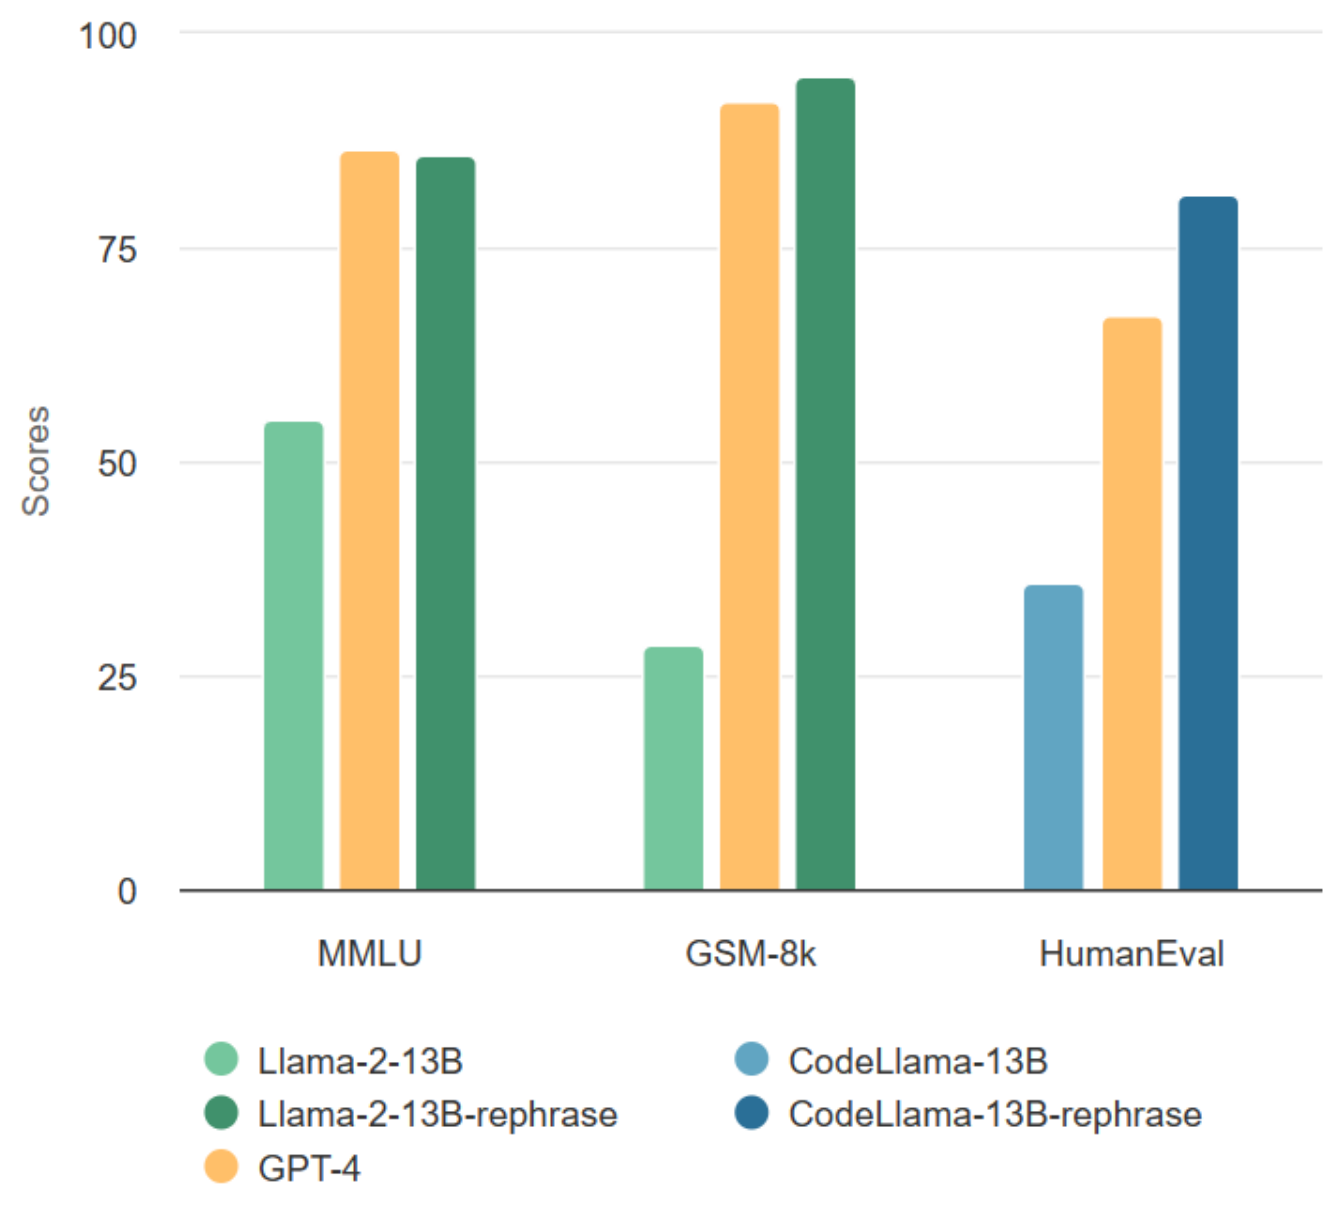
\includegraphics[width=\columnwidth]{high_chart_v11.png} % Replace "high_chart_v11.png" with your image filename
\caption{After fine-tuned on rephrased samples, Llama 2 and CodeLlama achieve performance on par with GPT-4.}
\vspace{-20pt}
\label{fig:benchmark_summary}
\end{figure}

% 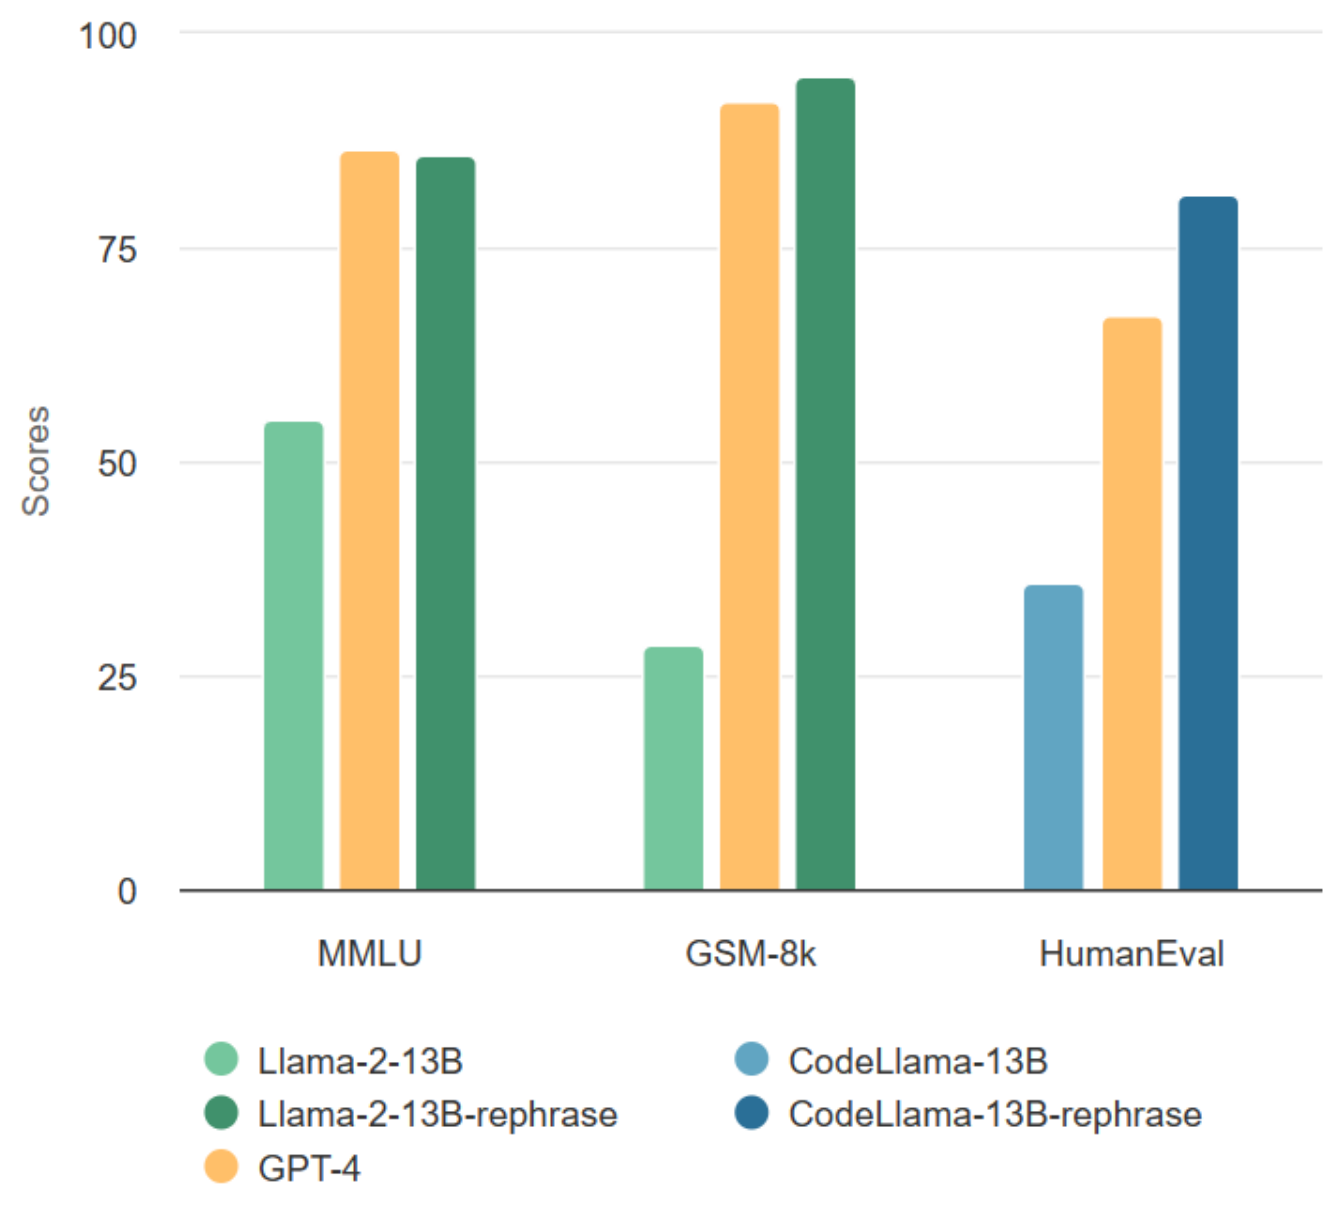
\includegraphics[width=\columnwidth]{high_chart_v11.png} % Replace "example-image" with your image filename
% \captionof{figure}{After fine-tuned on rephrased samples, Llama 2 and CodeLlama achieve performance on par with GPT-4.}
% \label{fig:benchmark_summary}

% \begin{figure}[t]
% 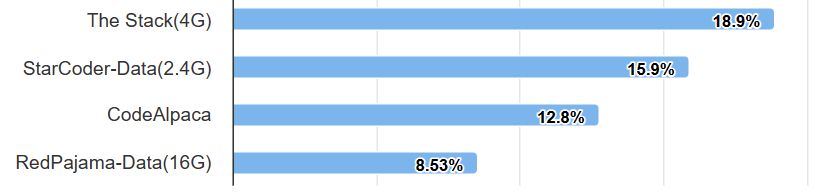
\includegraphics{high_bar_v7.png}
% \vspace{-10pt}
% \caption{The contamination percentage of HumanEval test cases in each training dataset.}
% \vspace{-15pt}
% \label{fig:dataset_summary}
% \end{figure}

% 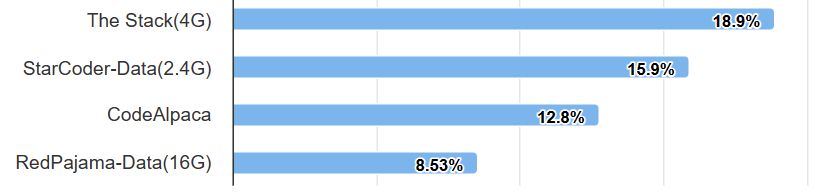
\includegraphics[width=\columnwidth]{high_bar_v7.png} % Replace "example-image" with your image filename
% \captionof{figure}{The contamination percentage of HumanEval test cases in each training dataset.}
% \label{fig:dataset_summary}

\begin{figure}[h!]
\centering
%\vspace{-5pt}
%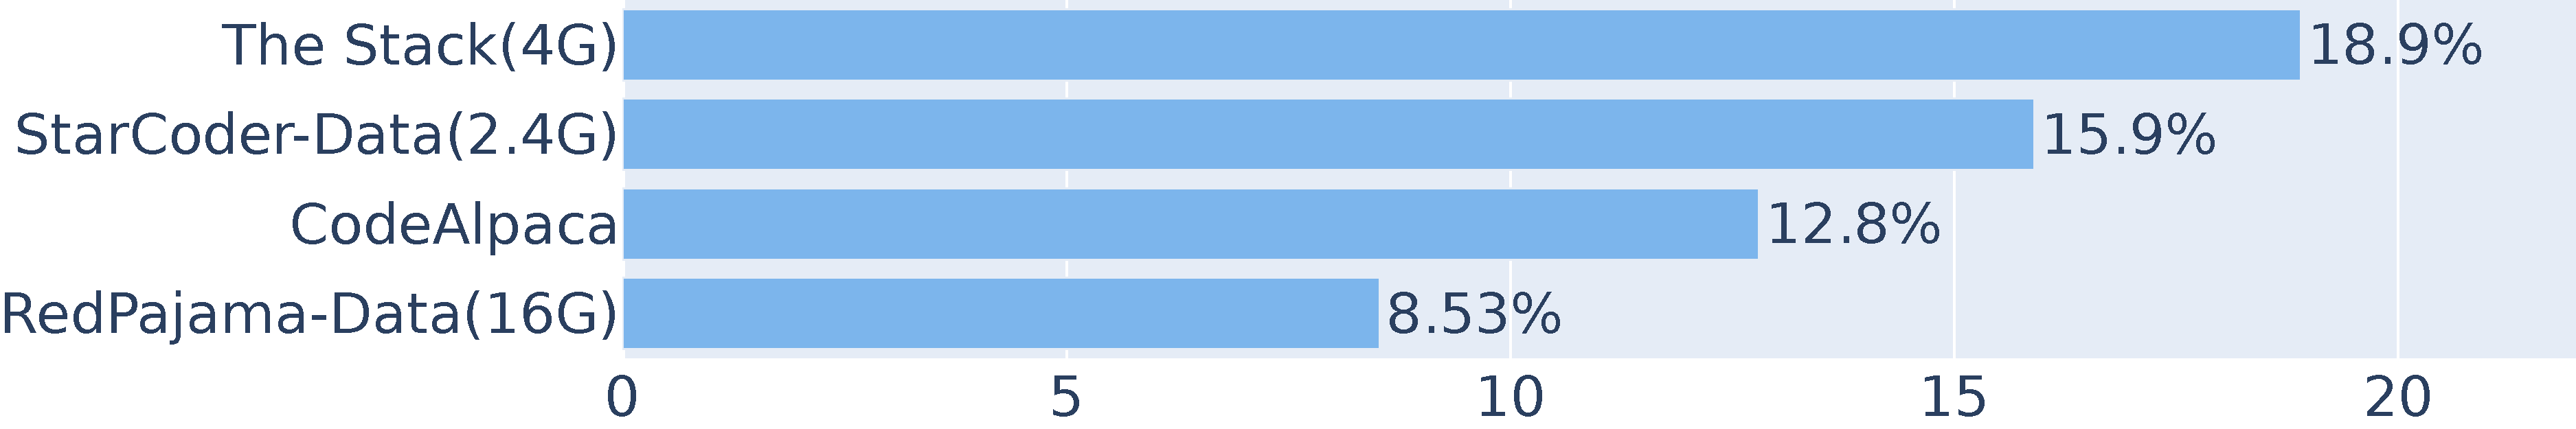
\includegraphics[width=\columnwidth]{fig1.pdf}
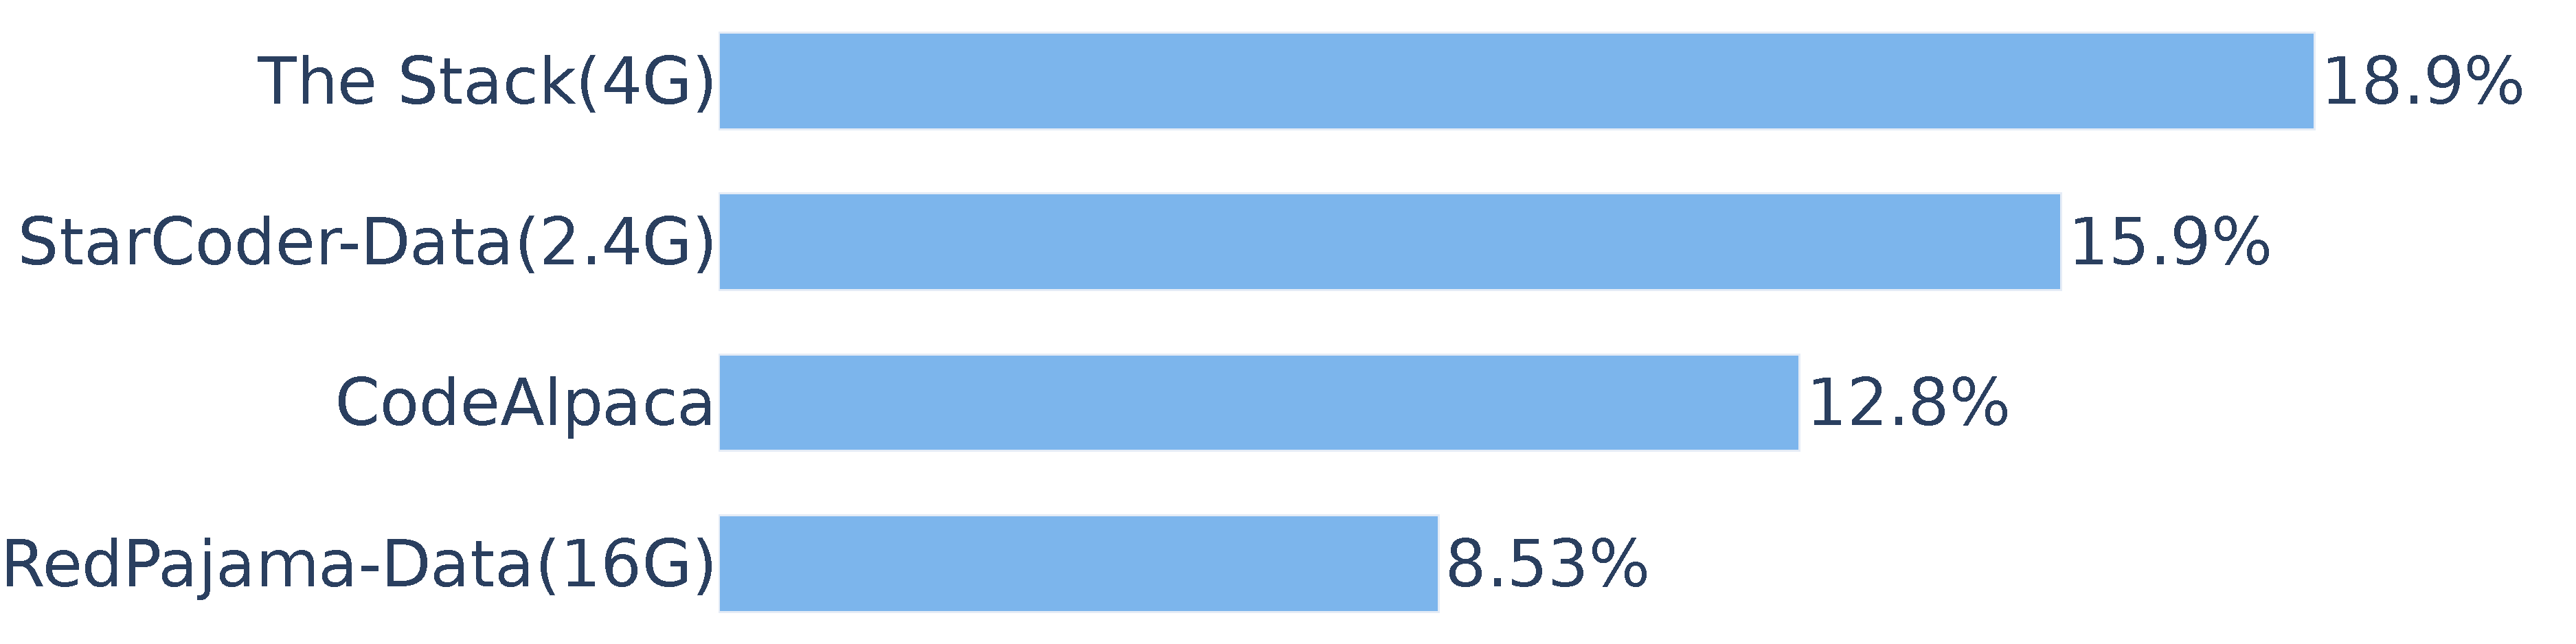
\includegraphics[width=\columnwidth]{humanevel_contamination.pdf}
\vspace{-15pt}
\caption{The contamination percentage of HumanEval benchmark in each training dataset. Note that The Stack (4G), StarCoder-Data (2.4G), and RedPajama-Data (16G) are subsets.}
\vspace{-10pt}
\label{fig:dataset_summary}
\end{figure}



% Two methods: 1. enhancing detection methods 2. one-time exam
% For method 1, we propose the LLM decontaminator. Describe what the method is. Highlight difference. Then results.

% For method 2, we endorse dynamic and live benchmarks. Call for community actions. Notable examples are DynaBench, Arena, and Kaggle competitions.

% Two strategies may be used to solve the problem of benchmark vulnerability: improving detection techniques and implementing live benchmarks.\ion{What are live benchmarks? Can we just use the same terminology, e.g., one-time exams/questions?}

% To enhance the capability of contamination detection, we propose the LLM decontaminator in section ~\ref{sec:llm-decontaminator}, which successfully detects rephrased samples.
% We use embedding similarity search to get the top-k training cases with the highest similarity for each test case in the benchmark. Then, we check each pair for contamination using a powerful LLM like GPT-4.
% The LLM decontaminator outperforms all existing detection methods on rephrased samples.
% In open fine-tuning datasets like FLAN~\citep{longpre2023flan}, CodeAlpaca~\citep{codealpaca}, and MATH~\citep{hendrycksmath2021}, we identify some rephrased samples. Notably, CodeAlpaca has a number of 12.8\% rephrased samples on HumanEval.
% Additionally, the pretraining dataset exhibits possible contamination. We detect 8.53\% of HumanEval rephrased samples within a 16G subset of RedPajama-Data-1T~\citep{together2023redpajama}.

% In FLAN, CodeAlpaca, and MATH, we found many test scenarios that resembled the rephrase attack by using the LLM decontaminator on open datasets.
% We used the LLM decontaminator to find rephrase contamination in a number of well-known real-world datasets, including FLAN, CodeAlpaca, and MATH. CodeAlpaca stood out for having a rephrase contamination rate of over 12.8\% on HumanEval, highlighting how common the problem is.

% In conclusion, we urge the community to employ the LLM Decontaminator when creating datasets.

% Live benchmarks may offer a solution to the problem of unhidden test sets in LLM evaluation.
% Model developers cannot overfit the test cases of live benchmarks, as these benchmarks continually refresh their test cases.
% As a result, we urge the community to use live benchmarks to evaluate LLMs' capabilities. 
% Live benchmarks do not have fixed questions, so overfitting the test set becomes much more difficult. 
% Fortunately, recent works have shown the potential of live benchmarks. 
% Dynabench~\citep{kiela2021dynabench} introduces a human-and-model-in-the-loop approach, facilitating the creation of more robust and informative benchmarks.
% Additionally, Chatbot Arena compares model capabilities from users' feedback, offering insights into their performance in real-world tasks. 
% We urge the community to set up contests similar to LeetCode's weekly competitions, thereby expanding the options for live benchmarking.
% \weilin{need to rewrite}

% In the future, there are some possible solutions to reduce the risk of contamination. 
% One approach is to employ more robust contamination detection methods to minimize unintentional contamination. Adopting one-time exams is another way to reflect a model's abilities. We introduce the LLM decontaminator and urge the community to set up evaluation criteria similar to those of Kaggle and Leetcode competitions. 

% \todo{one-time exams, highlight our decontaminator}

% In conclusion, we recommend that future benchmarks adopt a one-time exam approach, which can fundamentally eliminate both intentional and unintentional contamination. We urge the community to employ the LLM Decontaminator when creating datasets. Other forms of contamination besides rephrase attack might exist, necessitating a rethinking of potential weaknesses. It is possible to enhance existing benchmarks by perturbing them. 

% Model developers may simply overfit test sets for already-existing static benchmarks. As a result, improving detection techniques fall short in addressing deliberate contamination. As a result, we urge the community to use real benchmarks to assess the model capabilities. Given that live benchmarks don't have predetermined questions, overfitting to the test set becomes much more difficult. Static benchmarks may be replaced with Dynabench, and Chatbot Arena is skilled at facilitating assessments utilizing human-in-the-loop techniques. In addition, the community could set up contests to evaluate LLMs, offering a more realistic depiction of a model's genuine capabilities, similar to Leetcode's weekly challenges.
